\documentclass[conference]{IEEEtran}
\IEEEoverridecommandlockouts

\usepackage[utf8]{inputenc}
\usepackage[T1]{fontenc}
\usepackage[spanish,es-nodecimaldot,es-noshorthands,es-tabla]{babel}
\usepackage{amsmath,amssymb}
\usepackage{graphicx}
\usepackage{booktabs}
\usepackage{multirow}
\usepackage{url}
\usepackage{cite}
\usepackage{xcolor}
\usepackage{listings}

\graphicspath{{figuras/}}

\lstset{
  basicstyle=\ttfamily\scriptsize,
  breaklines=true,
  frame=single,
  columns=fullflexible,
  keepspaces=true,
  language=Matlab,
  commentstyle=\color{gray},
  keywordstyle=\color{blue!60!black}
}

\def\BibTeX{{\rm B\kern-.05em{\sc i\kern-.025em b}\kern-.08em T\kern-.1667em\lower.7ex\hbox{E}\kern-.125emX}}

\begin{document}

\title{Perceptr\'on simple y Adaline: implementaci\'on parametrizable en MATLAB y evaluaci\'on sobre compuertas l\'ogicas, Iris y autenticaci\'on de billetes}

\author{\IEEEauthorblockN{Sergio Duarte}
\IEEEauthorblockA{\textit{Maestr\'ia, Inteligencia Computacional Aplicada}\\
sergioduartedev@gmail.com}}

\maketitle

\begin{abstract}
Este trabajo implementa en MATLAB una red de una sola neurona y una sola capa bajo dos modelos cl\'asicos: el perceptr\'on simple, con tres reglas de correcci\'on de pesos seleccionables, y el Adaline, con la regla delta sobre la salida lineal. Ambas implementaciones son completamente parametrizables en n\'umero de entradas, umbral, factor de aprendizaje, codificaci\'on de la salida y criterio de parada. Los modelos se eval\'uan primero sobre compuertas AND y OR de 2, 3 y 4 entradas, midiendo el n\'umero de \'epocas hasta convergencia sobre 20 inicializaciones aleatorias, y luego sobre dos conjuntos de datos reales, Iris y \textit{Banknote Authentication}, particionados en proporciones 60-40, 70-30, 80-20 y 90-10. El perceptr\'on converge en todas las compuertas en menos de 20 \'epocas en promedio y alcanza 100\,\% de exactitud en el problema separable de Iris y hasta 99,3\,\% en billetes. El Adaline clasifica correctamente las compuertas en la mayor\'ia de los casos, aunque como minimiza el error cuadr\'atico y no el error de clasificaci\'on puede dejar patrones mal clasificados en las esquinas de la tabla de verdad, y en billetes alcanza 97,8\,\% siempre que las entradas est\'en escaladas: sin escalado el error diverge para $\alpha \geq 0{,}05$. Se documenta tambi\'en el efecto de la codificaci\'on de la salida, que anula la primera regla de aprendizaje cuando se usa $\{0,1\}$, y la imposibilidad de ambos modelos para resolver la XOR.
\end{abstract}

\begin{IEEEkeywords}
perceptr\'on, Adaline, regla delta, compuertas l\'ogicas, separabilidad lineal, MATLAB
\end{IEEEkeywords}

\section{Introducci\'on}

El perceptr\'on de Rosenblatt \cite{rosenblatt1958} y el Adaline de Widrow y Hoff \cite{widrow1960} son los dos modelos de neurona artificial m\'as antiguos que todav\'ia se ense\~nan, y por una buena raz\'on: con una sola neurona ya aparecen todos los conceptos que despu\'es escalan a redes profundas, es decir, pesos, umbral, funci\'on de activaci\'on, regla de aprendizaje, factor de aprendizaje, \'epocas y criterio de parada. La diferencia entre los dos modelos es sutil pero importante. El perceptr\'on corrige los pesos a partir del error de la salida binaria, de modo que solo corrige cuando se equivoca; el Adaline corrige a partir del error de la salida lineal, de modo que sigue ajustando aunque ya clasifique bien, buscando que la salida lineal se acerque al valor deseado.

Este documento corresponde al Taller 1 de la asignatura Inteligencia Computacional Aplicada y cubre sus doce puntos. Los puntos 1 a 6 piden un perceptr\'on parametrizable, probarlo en compuertas AND y OR de 2, 3 y 4 entradas, y despu\'es sobre particiones del conjunto Iris y del conjunto de autenticaci\'on de billetes. Los puntos 7 a 12 repiten lo mismo con el Adaline. Todo el c\'odigo est\'a en \textit{live scripts} de MATLAB \cite{matlab2026}, uno por bloque del taller, y las funciones de los dos modelos est\'an en archivos aparte para reutilizarlas.

El resto del documento se organiza as\'i. La secci\'on \ref{sec:marco} resume los dos modelos y sus reglas de aprendizaje. La secci\'on \ref{sec:metodo} describe la implementaci\'on, los conjuntos de datos y el protocolo experimental. La secci\'on \ref{sec:resultados} presenta los resultados, primero del perceptr\'on y luego del Adaline. La secci\'on \ref{sec:discusion} discute lo que sali\'o distinto de lo esperado y la secci\'on \ref{sec:conclusiones} cierra.

\section{Marco te\'orico}
\label{sec:marco}

\subsection{Perceptr\'on simple}

La neurona recibe $n$ entradas $x_1,\dots,x_n$ y una entrada constante igual a 1 cuyo peso $w_0$ hace de sesgo. La suma ponderada es
\begin{equation}
  z = w_0 + \sum_{i=1}^{n} w_i x_i ,
\end{equation}
y la salida se obtiene con una funci\'on escal\'on respecto de un umbral $\theta$:
\begin{equation}
  Y(x) = \begin{cases} y_{\max} & \text{si } z > \theta \\ y_{\min} & \text{en otro caso} \end{cases}
\end{equation}
donde $\{y_{\min}, y_{\max}\}$ es la codificaci\'on elegida para la salida, t\'ipicamente $\{-1,1\}$ o $\{0,1\}$.

El taller pide que el script permita elegir entre tres formas de correcci\'on de los pesos:
\begin{align}
  \Delta W_i &= d(x)\, X_i \label{eq:r1} \\
  \Delta W_i &= [d(x) - Y(x)]\, X_i \label{eq:r2} \\
  \Delta W_i &= \alpha\, [d(x) - Y(x)]\, X_i \label{eq:r3}
\end{align}
con $d(x)$ la salida deseada, $Y(x)$ la generada y $\alpha$ el factor relativo de aprendizaje, y el ajuste siempre es $W_i^{*} = W_i + \Delta W_i$. La regla \eqref{eq:r1} es la de tipo hebbiano vista en clase, se aplica solo cuando hay error y no usa la salida del modelo; la \eqref{eq:r2} es la regla del perceptr\'on original con $\alpha = 1$; la \eqref{eq:r3} es la misma con factor de aprendizaje. El teorema de convergencia del perceptr\'on garantiza que, si las clases son linealmente separables, la regla \eqref{eq:r3} encuentra un hiperplano separador en un n\'umero finito de correcciones \cite{haykin2009}.

\subsection{Adaline y regla delta}

El Adaline usa la misma suma ponderada, pero el error se calcula sobre la salida lineal $y = z$ y no sobre la salida del escal\'on. La regla delta minimiza el error cuadr\'atico por descenso de gradiente:
\begin{equation}
  \Delta W_i = \alpha\, [d(x) - y]\, X_i, \qquad \Delta \theta = \alpha\, [d(x) - y] ,
  \label{eq:delta}
\end{equation}
y el entrenamiento se detiene cuando el error cuadr\'atico de la \'epoca
\begin{equation}
  EC = \frac{1}{2}\sum_{k=1}^{Q} \varepsilon_k^2, \qquad \varepsilon_k = d^{(k)} - y^{(k)}
  \label{eq:ec}
\end{equation}
baja de un valor permitido, con $Q$ el n\'umero de patrones. Para clasificar, la salida lineal se pasa por un escal\'on con umbral $\theta$, en este trabajo $\theta = 0{,}5$ para salidas en $\{0,1\}$. Como la regla delta es un descenso de gradiente, el factor $\alpha$ tiene un l\'imite de estabilidad: si es demasiado grande el error crece en vez de bajar \cite{haykin2009}.

\subsection{Separabilidad lineal}

Una sola neurona con escal\'on solo puede representar funciones cuyas clases se separan con un hiperplano. Las compuertas AND y OR de cualquier n\'umero de entradas son linealmente separables; la XOR no lo es \cite{minsky1969}. En Iris, la clase \textit{setosa} es separable de las otras dos, mientras que \textit{versicolor} y \textit{virginica} se traslapan \cite{fisher1936}. Estas propiedades se usan aqu\'i como casos de prueba positivos y negativos.

\section{Metodolog\'ia}
\label{sec:metodo}

\subsection{Implementaci\'on}

Se escribieron dos funciones, \texttt{perceptron.m} y \texttt{adaline.m}, con la misma interfaz: reciben la matriz de patrones $X$ ($N \times n$), el vector de salidas deseadas $d$ y una estructura de opciones. La Tabla \ref{tab:params} lista los par\'ametros. Cada funci\'on devuelve los pesos, el sesgo y una estructura con el hist\'orico de la corrida. El sesgo se implementa como el peso $w_0$ de una entrada constante 1, que es exactamente el modelo de la figura del taller. Los pesos iniciales se toman de una distribuci\'on uniforme en $[0,1]$ a partir de una semilla, para que cualquier corrida sea reproducible. Una funci\'on auxiliar \texttt{predecir.m} aplica la suma ponderada y el escal\'on, y sirve igual para los dos modelos.

\begin{table}[!t]
\caption{Par\'ametros de las dos funciones}
\label{tab:params}
\centering
\small
\begin{tabular}{@{}lll@{}}
\toprule
Par\'ametro & Perceptr\'on & Adaline \\
\midrule
N\'umero de entradas & impl\'icito en $X$ & impl\'icito en $X$ \\
Regla de correcci\'on & 1, 2 o 3 & solo \eqref{eq:delta} \\
Factor $\alpha$ & s\'i & s\'i \\
Umbral $\theta$ & del escal\'on & del escal\'on al clasificar \\
Codificaci\'on de salida & $[y_{\min}, y_{\max}]$ & $[y_{\min}, y_{\max}]$ \\
Criterio de parada & \'epoca sin errores & $EC$ o $|\Delta EC|$ m\'inimos \\
Tope de \'epocas & s\'i & s\'i \\
Semilla & s\'i & s\'i \\
\bottomrule
\end{tabular}
\end{table}

En el perceptr\'on una \'epoca es una pasada por todos los patrones, y se declara convergencia cuando una \'epoca completa no requiere ninguna correcci\'on, lo que equivale al contador \texttt{aux} del c\'odigo de clase. En el Adaline se recorren los patrones uno a uno corrigiendo tras cada uno, como en el \texttt{codigo\_Adaline} de clase, y al final de la \'epoca se calcula \eqref{eq:ec}. Hizo falta un segundo criterio de parada, adem\'as del error m\'inimo: con una tabla de verdad la salida lineal nunca calza exactamente con los ceros y unos deseados, el $EC$ se estanca en un valor positivo y con solo el error m\'inimo el entrenamiento nunca terminar\'ia. Por eso tambi\'en se detiene cuando el cambio del $EC$ entre dos \'epocas consecutivas cae por debajo de una tolerancia, por defecto $10^{-6}$.

\subsection{Conjuntos de datos}

\textbf{Compuertas.} La funci\'on \texttt{compuerta.m} genera la tabla de verdad completa de AND, OR o XOR para $n$ entradas en $\{0,1\}$, con la salida codificada seg\'un se pida. Para $n = 2, 3, 4$ hay $4$, $8$ y $16$ patrones.

\textbf{Iris.} 150 flores, cuatro medidas en cent\'imetros y tres especies de 50 ejemplares cada una \cite{fisher1936}. Como la neurona es una sola, se arman dos problemas binarios: (A) \textit{setosa} contra las otras dos, que es linealmente separable, y (B) \textit{versicolor} contra \textit{virginica}, que no lo es.

\textbf{Banknote.} 1372 billetes descritos por cuatro estad\'isticos de la transformada \textit{wavelet} de su imagen: varianza, asimetr\'ia, curtosis y entrop\'ia. La clase indica si el billete es aut\'entico (762 casos) o falso (610) \cite{lohweg2013}. Las cuatro variables est\'an en escalas distintas; la curtosis, por ejemplo, va de $-5{,}3$ a $17{,}9$ mientras la entrop\'ia va de $-8{,}5$ a $2{,}4$.

\subsection{Particiones}

Siguiendo el script \texttt{Dataset\_train\_test} de clase, cada conjunto se mezcla una sola vez con \texttt{randperm} y semilla fija, y se corta en las proporciones 60-40, 70-30, 80-20 y 90-10. La \'unica modificaci\'on al script original fue redondear el punto de corte, porque $0{,}9 \times 1372 = 1234{,}8$ no sirve como \'indice. En Iris las particiones tienen 90, 105, 120 y 135 ejemplos de entrenamiento; en billetes 823, 960, 1098 y 1235. Las entradas se escalan al rango $[0,1]$ con los m\'inimos y m\'aximos del conjunto de entrenamiento, y esos mismos valores se aplican al de prueba. En billetes se entrena adem\'as sin escalar para medir el efecto.

\subsection{Protocolo experimental}

En compuertas, como el resultado depende de los pesos iniciales, cada combinaci\'on de compuerta, n\'umero de entradas y par\'ametro se repite con 20 semillas y se reporta el promedio de \'epocas junto con el porcentaje de corridas que convergieron. En los conjuntos reales se usa una semilla y se reporta la exactitud en entrenamiento y en prueba, las \'epocas y si convergi\'o. Los valores de $\alpha$ explorados son $\{0{,}01, 0{,}05, 0{,}1, 0{,}3, 0{,}5, 1\}$ para el perceptr\'on y $\{0{,}001, 0{,}01, 0{,}05, 0{,}1, 0{,}2, 0{,}5, 1\}$ para el Adaline en compuertas, con rangos m\'as bajos en billetes por la escala de las entradas. El tope de \'epocas es 100 en compuertas para el perceptr\'on, 1000 para el Adaline, y 200 y 500 respectivamente en los conjuntos reales.

\section{Resultados}
\label{sec:resultados}

\subsection{Perceptr\'on en compuertas}

La Fig. \ref{fig:fronteras} muestra las fronteras aprendidas para AND y OR de dos entradas con la regla \eqref{eq:r3}, $\alpha = 0{,}1$ y semilla 1. El perceptr\'on converge en 2 \'epocas en ambos casos. La Tabla \ref{tab:reglas} resume el comportamiento de las tres reglas en las seis compuertas con 20 semillas: todas convergen el 100\,\% de las veces y el n\'umero de \'epocas crece con el n\'umero de entradas, sobre todo en la AND, que con 4 entradas necesita entre 14 y 18 \'epocas en promedio frente a 4 o 6 de la OR. Entre reglas no hay diferencias grandes cuando la salida se codifica en $\{-1,1\}$; la regla \eqref{eq:r3} es ligeramente mejor en la AND de 4 entradas (14,0 contra 17,5 y 18,0).

\begin{figure}[!t]
\centering
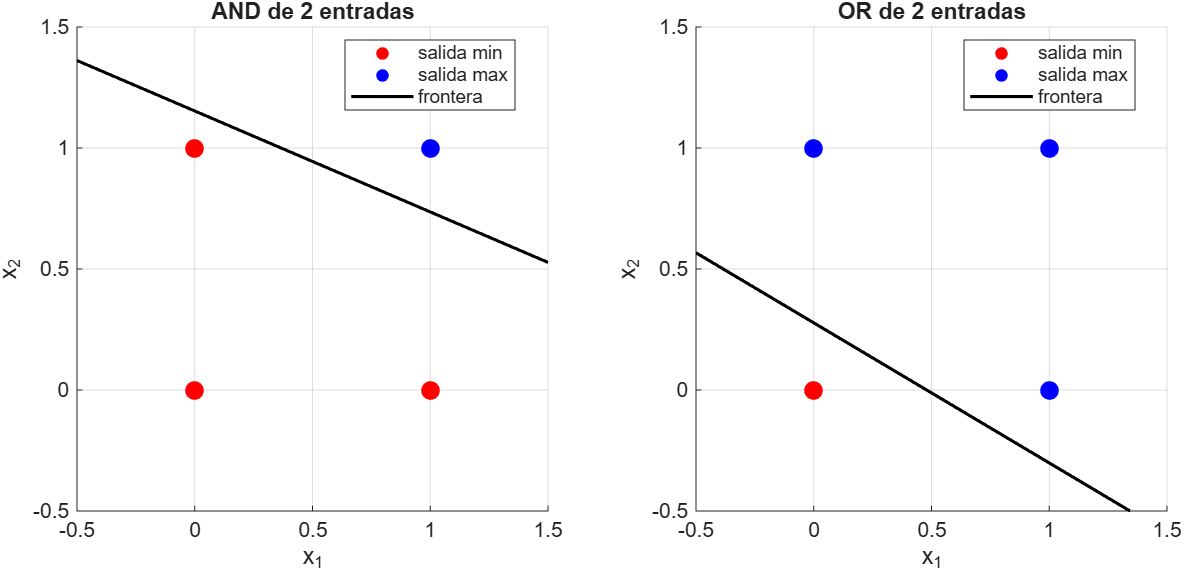
\includegraphics[width=\columnwidth]{perc_fronteras}
\caption{Fronteras de decisi\'on aprendidas por el perceptr\'on para AND y OR de dos entradas (regla 3, $\alpha = 0{,}1$, $\theta = 0$).}
\label{fig:fronteras}
\end{figure}

\begin{table}[!t]
\caption{Perceptr\'on: \'epocas promedio (m\'inimo--m\'aximo) hasta convergencia con las tres reglas, 20 semillas, $\alpha = 0{,}1$, $\theta = 0$, salida en $\{-1,1\}$. Convergi\'o el 100\,\% de las corridas en todos los casos.}
\label{tab:reglas}
\centering
\small
\begin{tabular}{@{}llccc@{}}
\toprule
Compuerta & $n$ & Regla 1 & Regla 2 & Regla 3 \\
\midrule
AND & 2 & 4,6 (2--8)   & 4,8 (2--6)   & 4,9 (2--7) \\
AND & 3 & 7,8 (2--15)  & 8,0 (2--18)  & 7,4 (2--14) \\
AND & 4 & 17,5 (4--31) & 18,0 (7--31) & 14,0 (3--34) \\
OR  & 2 & 3,0 (2--4)   & 4,0 (4--4)   & 4,6 (2--6) \\
OR  & 3 & 3,7 (2--5)   & 5,0 (5--5)   & 4,0 (2--6) \\
OR  & 4 & 4,2 (2--6)   & 6,0 (6--6)   & 4,2 (2--6) \\
\bottomrule
\end{tabular}
\end{table}

El efecto del factor de aprendizaje se muestra en la Fig. \ref{fig:perc_alpha} y la Tabla \ref{tab:perc_alpha}. Con $\alpha = 0{,}01$ el perceptr\'on necesita entre 18 y 28 \'epocas porque cada correcci\'on es muy peque\~na frente a los pesos iniciales, que est\'an en $[0,1]$. A partir de $\alpha = 0{,}1$ las \'epocas se estabilizan y ya no bajan m\'as; con $\alpha = 1$ incluso suben un poco en la OR. En el perceptr\'on no hay divergencia con $\alpha$ grande, porque la correcci\'on solo se aplica cuando hay error y siempre en la direcci\'on correcta.

\begin{figure}[!t]
\centering
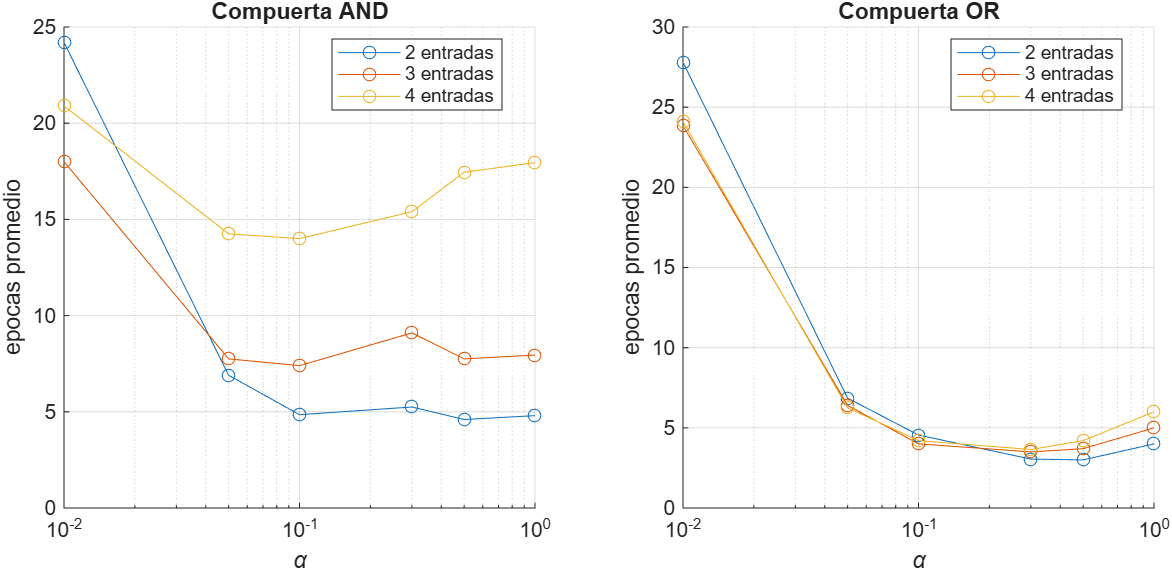
\includegraphics[width=\columnwidth]{perc_alpha}
\caption{\'Epocas promedio hasta convergencia del perceptr\'on (regla 3) en funci\'on de $\alpha$ para AND y OR de 2, 3 y 4 entradas, 20 semillas.}
\label{fig:perc_alpha}
\end{figure}

\begin{table}[!t]
\caption{Perceptr\'on, regla 3: \'epocas promedio seg\'un $\alpha$, 20 semillas. Todas las corridas convergieron.}
\label{tab:perc_alpha}
\centering
\small
\begin{tabular}{@{}lccccccc@{}}
\toprule
 & $n$ & 0,01 & 0,05 & 0,1 & 0,3 & 0,5 & 1 \\
\midrule
AND & 2 & 24,2 & 6,9  & 4,9  & 5,3  & 4,6  & 4,8 \\
AND & 3 & 18,0 & 7,8  & 7,4  & 9,1  & 7,8  & 8,0 \\
AND & 4 & 20,9 & 14,3 & 14,0 & 15,4 & 17,5 & 18,0 \\
OR  & 2 & 27,8 & 6,9  & 4,6  & 3,1  & 3,0  & 4,0 \\
OR  & 3 & 23,9 & 6,4  & 4,0  & 3,5  & 3,7  & 5,0 \\
OR  & 4 & 24,1 & 6,3  & 4,2  & 3,7  & 4,2  & 6,0 \\
\bottomrule
\end{tabular}
\end{table}

El umbral $\theta$ tambi\'en influye. Para las compuertas de dos entradas, con $\theta = -1$ la AND tarda 8,0 \'epocas y la OR 9,6; con $\theta = 0$ tardan 4,9 y 4,6; con $\theta = 1$ tardan 2,8 y 2,0. Como los pesos iniciales son positivos, un umbral positivo deja de entrada la neurona apagada para los patrones con pocas entradas activas, que es lo que tanto la AND como la OR necesitan para la mayor\'ia de sus filas, y por eso hay menos que corregir.

La codificaci\'on de la salida result\'o ser el par\'ametro con el efecto m\'as dr\'astico, y se muestra en la Tabla \ref{tab:codif}. Con salida en $\{-1,1\}$ las tres reglas convergen. Con salida en $\{0,1\}$ las reglas \eqref{eq:r2} y \eqref{eq:r3} siguen convergiendo, pero la regla \eqref{eq:r1} no converge nunca en 100 \'epocas. La raz\'on es directa: cuando la salida deseada es 0, $\Delta W_i = d(x) X_i = 0$, as\'i que la neurona no recibe ninguna correcci\'on de los patrones que deber\'ian dar salida baja y solo aprende a activarse. Con $\{-1,1\}$ esos patrones s\'i empujan los pesos en direcci\'on negativa.

\begin{table}[!t]
\caption{Perceptr\'on de dos entradas: efecto de la codificaci\'on de la salida, 20 semillas, $\alpha = 0{,}1$.}
\label{tab:codif}
\centering
\small
\begin{tabular}{@{}llccc@{}}
\toprule
Salida & Compuerta & Regla & \'Epocas prom. & Convergi\'o \\
\midrule
$\{-1,1\}$ & AND & 1 & 4,6 & 100\,\% \\
$\{-1,1\}$ & AND & 2 & 4,8 & 100\,\% \\
$\{-1,1\}$ & AND & 3 & 4,9 & 100\,\% \\
$\{-1,1\}$ & OR  & 1 & 3,0 & 100\,\% \\
$\{-1,1\}$ & OR  & 2 & 4,0 & 100\,\% \\
$\{-1,1\}$ & OR  & 3 & 4,6 & 100\,\% \\
$\{0,1\}$  & AND & 1 & 100 & 0\,\% \\
$\{0,1\}$  & AND & 2 & 4,6 & 100\,\% \\
$\{0,1\}$  & AND & 3 & 6,9 & 100\,\% \\
$\{0,1\}$  & OR  & 1 & 100 & 0\,\% \\
$\{0,1\}$  & OR  & 2 & 3,0 & 100\,\% \\
$\{0,1\}$  & OR  & 3 & 6,9 & 100\,\% \\
\bottomrule
\end{tabular}
\end{table}

\subsection{Perceptr\'on en Iris}

La Tabla \ref{tab:perc_iris} resume las cuatro particiones promediando sobre los cinco valores de $\alpha$. En el problema A, \textit{setosa} contra el resto, el perceptr\'on converge siempre y clasifica el 100\,\% tanto en entrenamiento como en prueba en las cuatro particiones; el \'unico efecto de $\alpha$ es la velocidad, de 15 a 17 \'epocas con $\alpha = 0{,}01$ a 2 \'epocas con $\alpha \geq 0{,}5$. En el problema B el perceptr\'on casi nunca converge y agota las 200 \'epocas, con exactitud en entrenamiento entre 94,6 y 98,7\,\% y en prueba entre 87,5 y 100\,\%. La Fig. \ref{fig:iris_vv} muestra por qu\'e: en el plano largo y ancho del p\'etalo las dos clases se traslapan y ninguna recta las separa. Hubo tres casos en los que s\'i convergi\'o en el conjunto de entrenamiento, por ejemplo la partici\'on 60-40 con $\alpha = 0{,}1$ en 17 \'epocas con 100\,\% de acierto en entrenamiento, lo que indica que ese subconjunto particular s\'i era separable; en prueba, sin embargo, dio 93,2\,\%, igual que los casos que no convergieron. El 100\,\% de la partici\'on 90-10 corresponde a un conjunto de prueba de solo 10 flores y no debe leerse como una mejora real.

\begin{table}[!t]
\caption{Perceptr\'on en Iris: promedio sobre $\alpha \in \{0{,}01, 0{,}05, 0{,}1, 0{,}5, 1\}$. Exactitud en \%.}
\label{tab:perc_iris}
\centering
\small
\begin{tabular}{@{}llccc@{}}
\toprule
Problema & Partici\'on & \'Epocas & Entren. & Prueba \\
\midrule
A & 60-40 & 6,0   & 100,0 & 100,0 \\
A & 70-30 & 5,6   & 100,0 & 100,0 \\
A & 80-20 & 6,0   & 100,0 & 100,0 \\
A & 90-10 & 6,0   & 100,0 & 100,0 \\
B & 60-40 & 125,6 & 97,9  & 92,7 \\
B & 70-30 & 200,0 & 98,5  & 89,4 \\
B & 80-20 & 175,0 & 98,5  & 91,4 \\
B & 90-10 & 200,0 & 95,4  & 100,0 \\
\bottomrule
\end{tabular}
\end{table}

\begin{figure}[!t]
\centering
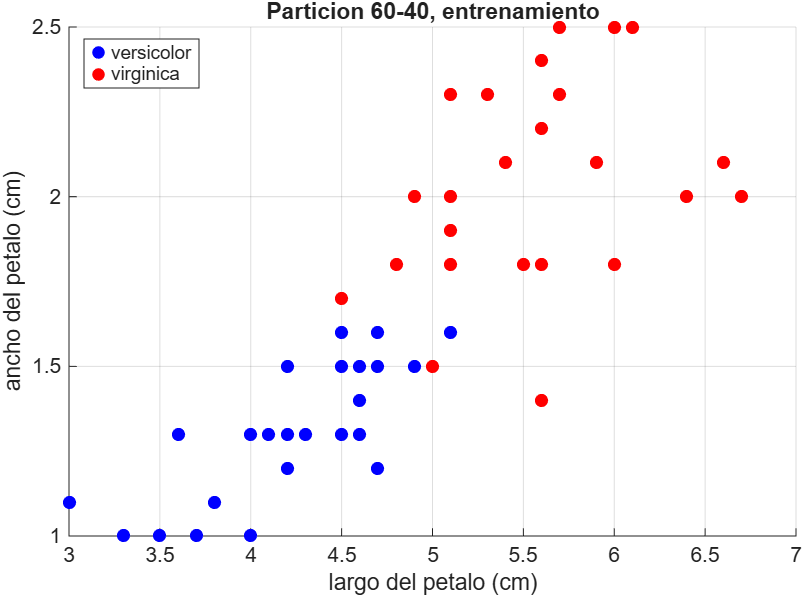
\includegraphics[width=0.85\columnwidth]{iris_versicolor_virginica}
\caption{Problema B de Iris en el plano largo y ancho del p\'etalo, partici\'on 60-40. Las clases se traslapan y el perceptr\'on no converge.}
\label{fig:iris_vv}
\end{figure}

\subsection{Perceptr\'on en billetes}

Con los cuatro atributos de la transformada \textit{wavelet} el perceptr\'on no converge en 200 \'epocas en ninguna de las 40 corridas, lo que indica que las dos clases no son perfectamente separables, pero la exactitud es alta y estable: entre 97,1 y 99,3\,\% en prueba. La Tabla \ref{tab:perc_bank} resume por partici\'on y escalado. El escalado al rango $[0,1]$ no ayuda al perceptr\'on, y de hecho la mejor exactitud, 99,3\,\% en la partici\'on 60-40 con $\alpha = 0{,}05$, se obtiene sin escalar. Esto es coherente con el modelo: el escal\'on solo mira el signo de la suma ponderada, as\'i que la escala de las entradas se compensa con la escala de los pesos. La Fig. \ref{fig:perc_bank} muestra las curvas de exactitud contra $\alpha$. En el mejor caso, de 549 billetes de prueba el perceptr\'on se equivoca en 4.

\begin{table}[!t]
\caption{Perceptr\'on en billetes: promedio sobre $\alpha \in \{0{,}01, 0{,}05, 0{,}1, 0{,}5, 1\}$. Ninguna corrida convergi\'o en 200 \'epocas. Exactitud en \%.}
\label{tab:perc_bank}
\centering
\small
\begin{tabular}{@{}llcc@{}}
\toprule
Escalado & Partici\'on & Entren. & Prueba \\
\midrule
no & 60-40 & 98,9 & 99,2 \\
no & 70-30 & 98,6 & 98,6 \\
no & 80-20 & 98,7 & 98,4 \\
no & 90-10 & 98,8 & 98,4 \\
s\'i & 60-40 & 98,6 & 98,1 \\
s\'i & 70-30 & 98,9 & 98,4 \\
s\'i & 80-20 & 98,9 & 98,5 \\
s\'i & 90-10 & 98,5 & 97,7 \\
\bottomrule
\end{tabular}
\end{table}

\begin{figure}[!t]
\centering
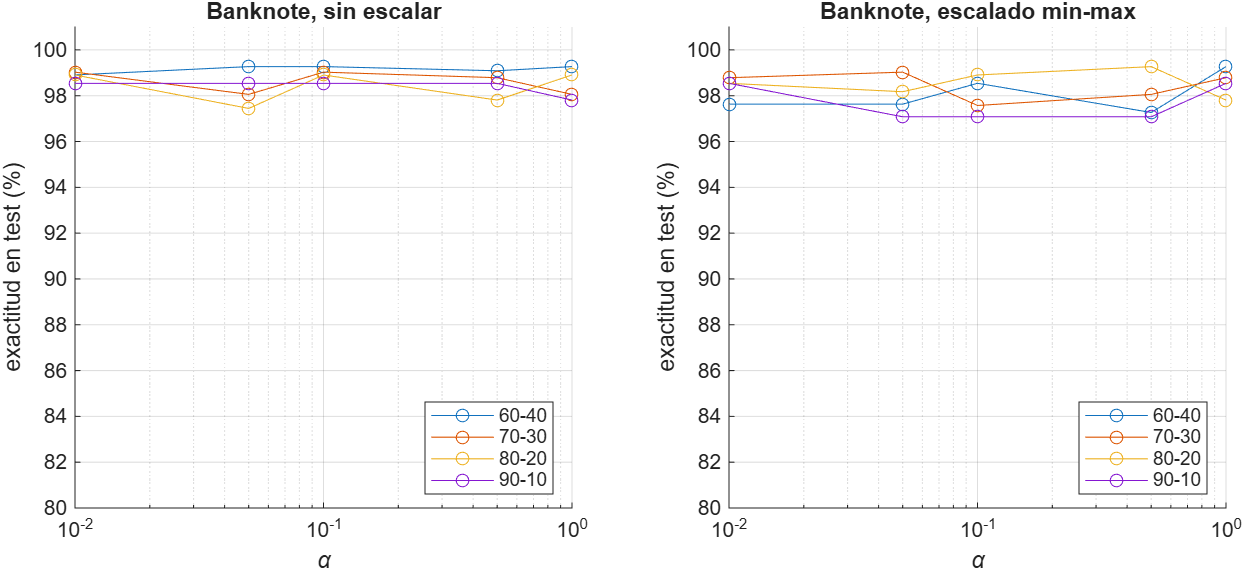
\includegraphics[width=\columnwidth]{perc_banknote}
\caption{Perceptr\'on en billetes: exactitud en prueba contra $\alpha$ para las cuatro particiones, sin escalar y con escalado min-max.}
\label{fig:perc_bank}
\end{figure}

\subsection{Adaline en compuertas}

La Fig. \ref{fig:ada_or2} muestra el Adaline en la OR de dos entradas con $\alpha = 0{,}05$. La salida lineal para los cuatro patrones queda en 0,26, 0,75, 0,73 y 1,23, y el escal\'on en 0,5 los clasifica todos bien. El $EC$ baja de forma mon\'otona y se estanca en 0,1385 despu\'es de 104 \'epocas: ese es el m\'inimo del error cuadr\'atico de una recta ajustada a esa tabla de verdad, y no es cero porque los cuatro puntos no est\'an sobre un plano. Aqu\'i se ve la diferencia de fondo con el perceptr\'on, que para en cuanto clasifica bien: el Adaline sigue afinando la salida lineal aunque la clasificaci\'on ya sea correcta.

\begin{figure}[!t]
\centering
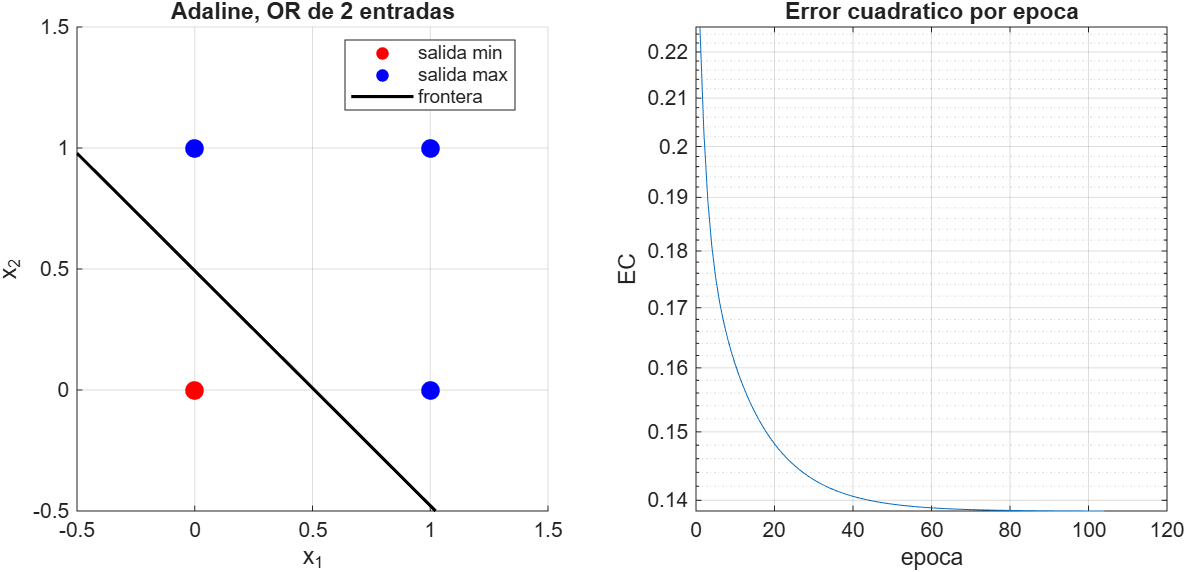
\includegraphics[width=\columnwidth]{ada_or2}
\caption{Adaline en la OR de dos entradas ($\alpha = 0{,}05$): frontera aprendida y error cuadr\'atico por \'epoca.}
\label{fig:ada_or2}
\end{figure}

La Tabla \ref{tab:ada_comp} resume las siete compuertas con los mismos par\'ametros. En todas el entrenamiento se detiene por la tolerancia de cambio entre 53 y 128 \'epocas. La exactitud es 100\,\% en AND y OR de 2 y 3 entradas, pero en la AND de 4 entradas clasifica mal un patr\'on de 16 (93,75\,\%) y en la OR de 3 entradas un patr\'on de 8 (87,5\,\%). Esto no es un error de implementaci\'on sino una propiedad del modelo: la regla delta minimiza el error cuadr\'atico de la salida lineal, y el plano que minimiza ese error no es necesariamente el que separa las clases. Al aumentar el n\'umero de entradas la tabla de verdad tiene m\'as esquinas y la recta de m\'inimos cuadrados queda m\'as lejos de algunas de ellas. Con $\alpha = 0{,}1$ la AND de 4 s\'i alcanza el 100\,\%, lo que muestra que la soluci\'on a la que se llega tambi\'en depende del camino. La XOR, como se esperaba, no se resuelve: el $EC$ se estanca en 0,554 y la exactitud es 25\,\%.

\begin{table}[!t]
\caption{Adaline en compuertas: $\alpha = 0{,}05$, tolerancia $10^{-6}$, umbral 0,5, semilla 1.}
\label{tab:ada_comp}
\centering
\small
\begin{tabular}{@{}llccc@{}}
\toprule
Compuerta & $n$ & \'Epocas & $EC$ final & Exactitud \\
\midrule
AND & 2 & 67  & 0,138 & 100\,\% \\
AND & 3 & 115 & 0,295 & 100\,\% \\
AND & 4 & 59  & 0,429 & 93,75\,\% \\
OR  & 2 & 104 & 0,139 & 100\,\% \\
OR  & 3 & 53  & 0,273 & 87,5\,\% \\
OR  & 4 & 86  & 0,370 & 93,75\,\% \\
XOR & 2 & 128 & 0,554 & 25\,\% \\
\bottomrule
\end{tabular}
\end{table}

El factor de aprendizaje tiene en el Adaline un comportamiento muy distinto al del perceptr\'on, y se resume en la Tabla \ref{tab:ada_alpha} y en la Fig. \ref{fig:ada_alpha}. Con $\alpha = 0{,}001$ el error baja tan despacio que no se estanca en 1000 \'epocas. Entre 0,01 y 0,2 el n\'umero de \'epocas cae de unas 300 a unas 40 y el $EC$ final se mantiene cerca del m\'inimo. Con $\alpha = 0{,}5$ el algoritmo para r\'apido pero en un $EC$ mayor, por ejemplo 0,5 en la AND de 2 y 1,81 en la AND de 4, y la exactitud cae a 75 y 56\,\%; y con $\alpha = 1$ el error diverge, llegando a $5 \times 10^{5}$ en dos entradas y a infinito en tres y cuatro. Es el l\'imite de estabilidad del descenso de gradiente: con un paso demasiado grande cada correcci\'on sobrepasa el m\'inimo y el error crece.

\begin{table}[!t]
\caption{Adaline: \'epocas hasta que el $EC$ deja de bajar, $EC$ final y exactitud seg\'un $\alpha$, para AND y OR de 2 y 4 entradas.}
\label{tab:ada_alpha}
\centering
\small
\begin{tabular}{@{}lccccccc@{}}
\toprule
 & 0,001 & 0,01 & 0,05 & 0,1 & 0,2 & 0,5 & 1 \\
\midrule
\multicolumn{8}{@{}l}{\textit{AND 2}} \\
\'Epocas & 1000 & 327 & 67 & 27 & 47 & 20 & 1000 \\
$EC$ & 0,129 & 0,128 & 0,138 & 0,154 & 0,195 & 0,500 & $5{\cdot}10^{5}$ \\
Exact. & 100 & 100 & 100 & 100 & 100 & 75 & 50 \\
\multicolumn{8}{@{}l}{\textit{AND 4}} \\
\'Epocas & 1000 & 186 & 59 & 42 & 35 & 30 & 96 \\
$EC$ & 0,346 & 0,359 & 0,429 & 0,531 & 0,762 & 1,807 & $\infty$ \\
Exact. & 93,8 & 93,8 & 93,8 & 100 & 81,3 & 56,3 & 6,3 \\
\multicolumn{8}{@{}l}{\textit{OR 2}} \\
\'Epocas & 1000 & 435 & 104 & 49 & 20 & 19 & 1000 \\
$EC$ & 0,133 & 0,128 & 0,139 & 0,154 & 0,195 & 0,500 & $5{\cdot}10^{5}$ \\
Exact. & 100 & 100 & 100 & 100 & 100 & 75 & 0 \\
\multicolumn{8}{@{}l}{\textit{OR 4}} \\
\'Epocas & 1000 & 237 & 86 & 51 & 34 & 23 & 96 \\
$EC$ & 0,356 & 0,349 & 0,370 & 0,394 & 0,435 & 0,655 & $\infty$ \\
Exact. & 93,8 & 93,8 & 93,8 & 93,8 & 93,8 & 93,8 & 6,3 \\
\bottomrule
\end{tabular}
\end{table}

\begin{figure}[!t]
\centering
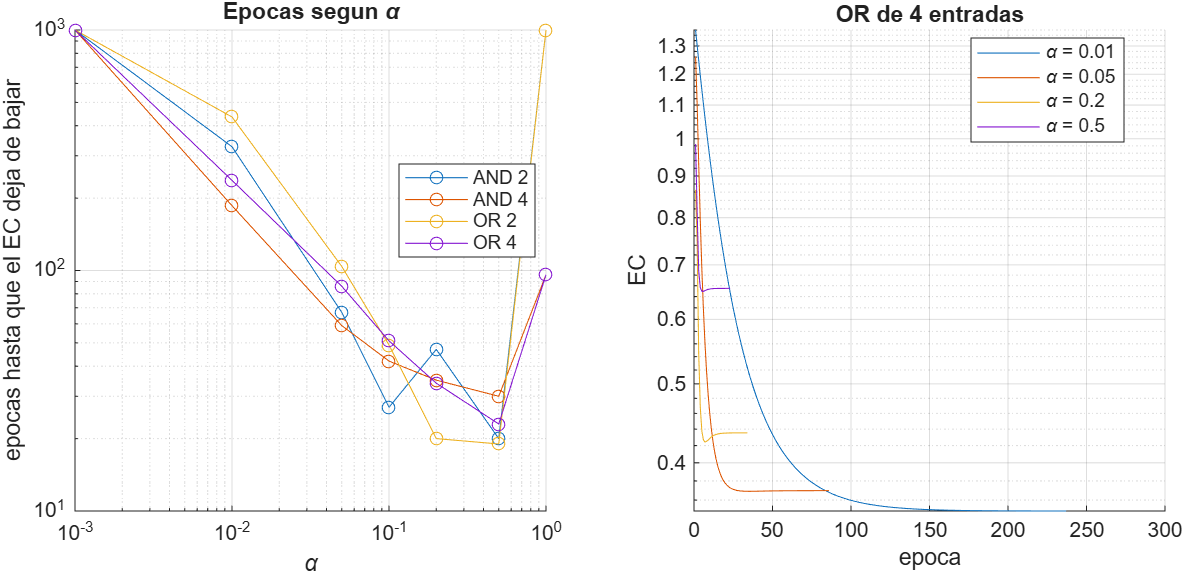
\includegraphics[width=\columnwidth]{ada_alpha}
\caption{Adaline: \'epocas hasta estancarse seg\'un $\alpha$ (izquierda) y curva del $EC$ en la OR de 4 entradas para cuatro valores de $\alpha$ (derecha).}
\label{fig:ada_alpha}
\end{figure}

La tolerancia de parada y el umbral del escal\'on se exploraron en la AND de dos entradas. Con tolerancia $10^{-2}$ el entrenamiento para en 6 \'epocas con $EC = 0{,}162$, con $10^{-4}$ en 34 \'epocas con $EC = 0{,}139$ y con $10^{-6}$ en 67 \'epocas con $EC = 0{,}1385$, que ya es el m\'inimo. La exactitud es 100\,\% con umbral 0,5 y 0,7 en todos los casos; con umbral 0,3 y tolerancia gruesa ($10^{-2}$ o $10^{-3}$) baja a 75\,\%, porque la salida lineal del patr\'on $(0,1)$ todav\'ia est\'a por encima de 0,3 cuando el entrenamiento se detiene temprano.

La Tabla \ref{tab:pva_comp} compara los dos modelos en las mismas compuertas, con $\alpha = 0{,}05$, salida en $\{0,1\}$ y umbral 0,5. El perceptr\'on converge en 2 a 7 \'epocas con 100\,\% en todas las compuertas separables; el Adaline gasta entre 53 y 115 \'epocas y en dos casos deja patrones mal clasificados. En la XOR ninguno de los dos funciona.

\begin{table}[!t]
\caption{Perceptr\'on (regla 3) contra Adaline en compuertas, $\alpha = 0{,}05$, salida $\{0,1\}$, umbral 0,5, semilla 1.}
\label{tab:pva_comp}
\centering
\small
\begin{tabular}{@{}llcccc@{}}
\toprule
 & & \multicolumn{2}{c}{Perceptr\'on} & \multicolumn{2}{c}{Adaline} \\
\cmidrule(lr){3-4} \cmidrule(lr){5-6}
Compuerta & $n$ & \'Epocas & Exact. & \'Epocas & Exact. \\
\midrule
AND & 2 & 4    & 100 & 67  & 100 \\
AND & 3 & 7    & 100 & 115 & 100 \\
AND & 4 & 6    & 100 & 59  & 93,75 \\
OR  & 2 & 2    & 100 & 104 & 100 \\
OR  & 3 & 3    & 100 & 53  & 87,5 \\
OR  & 4 & 5    & 100 & 86  & 93,75 \\
XOR & 2 & 1000 & 50  & 128 & 25 \\
\bottomrule
\end{tabular}
\end{table}

\subsection{Adaline en Iris}

La Tabla \ref{tab:ada_iris} resume los resultados con $\alpha \in \{0{,}001, 0{,}005, 0{,}01, 0{,}05, 0{,}1\}$. En el problema A el Adaline clasifica el 100\,\% en entrenamiento y prueba en las cuatro particiones, igual que el perceptr\'on, pero necesita cientos de \'epocas porque sigue reduciendo el $EC$ mucho despu\'es de que la clasificaci\'on ya es correcta; con los $\alpha$ m\'as peque\~nos ni siquiera se estanca en las 500 \'epocas de tope. En el problema B la exactitud en prueba va de 90,6 a 100\,\%, muy parecida a la del perceptr\'on, con la diferencia de que el Adaline s\'i se detiene de forma ordenada cuando el $EC$ deja de bajar, mientras que el perceptr\'on agotaba el tope de \'epocas sin converger. La Fig. \ref{fig:ada_iris_ec} muestra las dos curvas de error: en A el $EC$ baja hasta cerca de 1,0 y en B se queda en 1,4, que es el reflejo del traslape entre clases.

\begin{table}[!t]
\caption{Adaline en Iris: promedio sobre cinco valores de $\alpha$. Exactitud en \%.}
\label{tab:ada_iris}
\centering
\small
\begin{tabular}{@{}llcccc@{}}
\toprule
Problema & Partici\'on & \'Epocas & $EC$ final & Entren. & Prueba \\
\midrule
A & 60-40 & 467 & 0,97 & 100,0 & 100,0 \\
A & 70-30 & 451 & 1,13 & 100,0 & 100,0 \\
A & 80-20 & 446 & 1,32 & 100,0 & 100,0 \\
A & 90-10 & 431 & 1,49 & 100,0 & 100,0 \\
B & 60-40 & 398 & 1,46 & 98,2 & 93,6 \\
B & 70-30 & 381 & 1,73 & 98,5 & 90,6 \\
B & 80-20 & 353 & 2,40 & 98,0 & 94,3 \\
B & 90-10 & 359 & 2,67 & 97,0 & 100,0 \\
\bottomrule
\end{tabular}
\end{table}

\begin{figure}[!t]
\centering
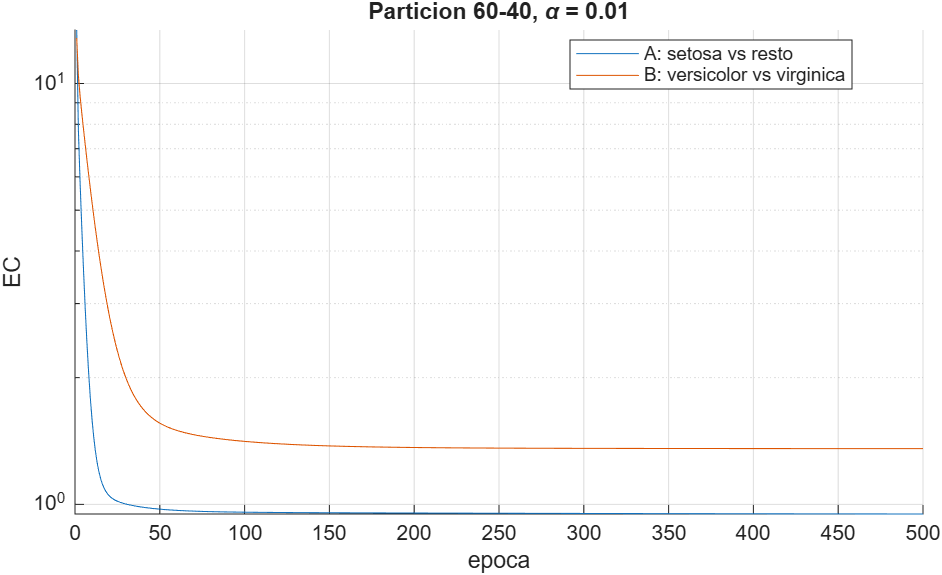
\includegraphics[width=0.9\columnwidth]{ada_iris_ec}
\caption{Adaline en Iris, partici\'on 60-40 y $\alpha = 0{,}01$: error cuadr\'atico por \'epoca en los dos problemas.}
\label{fig:ada_iris_ec}
\end{figure}

\subsection{Adaline en billetes}

Aqu\'i el escalado pasa de ser irrelevante a ser decisivo, y la Tabla \ref{tab:ada_bank} lo muestra. Sin escalar, con $\alpha = 0{,}05$ el error se dispara a infinito en una o dos \'epocas en las cuatro particiones y la exactitud cae al nivel del azar, entre 34 y 62\,\%; con $\alpha = 0{,}01$ el error ya no diverge pero queda alto y la exactitud baja a 92--97\,\%; solo con $\alpha \leq 0{,}001$ se obtienen resultados buenos, de 96,1 a 97,5\,\%. La causa es la curtosis, que llega a 17,9: en la regla delta la correcci\'on es proporcional a la entrada, y una entrada grande multiplica el paso efectivo. Con las entradas escaladas a $[0,1]$ todo $\alpha$ entre 0,001 y 0,05 da entre 95,9 y 97,8\,\%, y solo $\alpha = 10^{-4}$ es demasiado lento y se queda en 89--93\,\% al agotar las 500 \'epocas. La Fig. \ref{fig:ada_bank} muestra las dos situaciones y la Fig. \ref{fig:ada_bank_mejor} el mejor caso, la partici\'on 80-20 escalada con $\alpha = 0{,}005$, que llega a 97,8\,\% en prueba con 287 \'epocas.

\begin{table}[!t]
\caption{Adaline en billetes: exactitud en prueba (\%) por partici\'on y $\alpha$, sin escalar y con escalado min-max. Se marca con $\infty$ la divergencia del $EC$.}
\label{tab:ada_bank}
\centering
\small
\begin{tabular}{@{}llccccc@{}}
\toprule
Escalado & Partici\'on & $10^{-4}$ & $10^{-3}$ & $5{\cdot}10^{-3}$ & $10^{-2}$ & $5{\cdot}10^{-2}$ \\
\midrule
no & 60-40 & 96,7 & 97,5 & 96,5 & 94,0 & 36,1 ($\infty$) \\
no & 70-30 & 96,1 & 96,4 & 97,1 & 97,3 & 44,4 ($\infty$) \\
no & 80-20 & 97,4 & 97,4 & 96,4 & 92,3 & 34,3 ($\infty$) \\
no & 90-10 & 96,4 & 96,4 & 96,4 & 94,9 & 62,0 ($\infty$) \\
s\'i & 60-40 & 88,9 & 96,9 & 96,5 & 96,5 & 96,4 \\
s\'i & 70-30 & 90,8 & 96,1 & 96,1 & 96,1 & 95,9 \\
s\'i & 80-20 & 91,6 & 97,4 & 97,8 & 97,8 & 97,4 \\
s\'i & 90-10 & 93,4 & 96,4 & 96,4 & 96,4 & 96,4 \\
\bottomrule
\end{tabular}
\end{table}

\begin{figure}[!t]
\centering
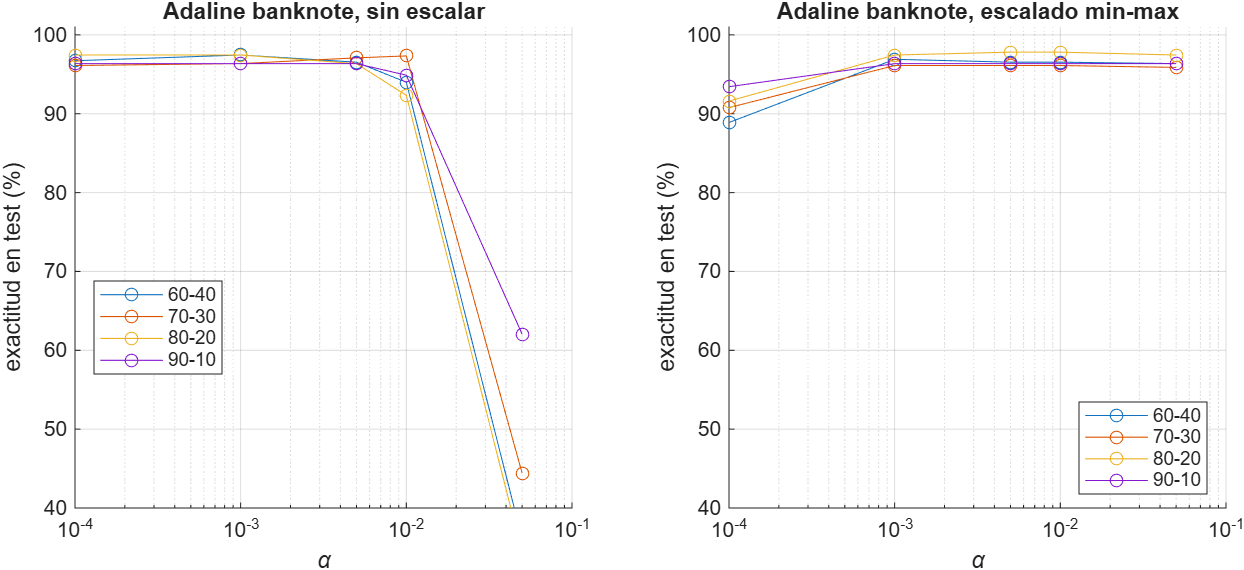
\includegraphics[width=\columnwidth]{ada_banknote}
\caption{Adaline en billetes: exactitud en prueba contra $\alpha$, sin escalar (izquierda) y con escalado (derecha). Sin escalar, $\alpha = 0{,}05$ diverge.}
\label{fig:ada_bank}
\end{figure}

\begin{figure}[!t]
\centering
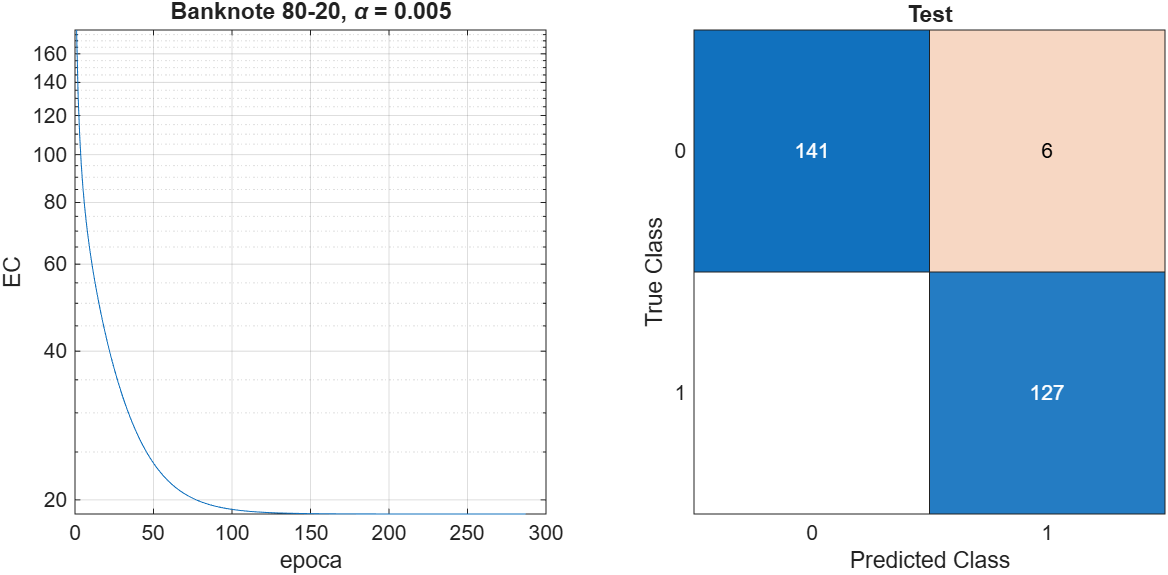
\includegraphics[width=\columnwidth]{ada_banknote_mejor}
\caption{Mejor Adaline en billetes (80-20, escalado, $\alpha = 0{,}005$): curva del $EC$ y matriz de confusi\'on en prueba.}
\label{fig:ada_bank_mejor}
\end{figure}

La Tabla \ref{tab:pva_bank} cierra la comparaci\'on entre los dos modelos sobre la partici\'on 80-20 escalada. El perceptr\'on obtiene entre 97,4 y 98,9\,\% pero nunca converge, y agota las 500 \'epocas para todo $\alpha$; el Adaline obtiene entre 97,4 y 97,8\,\% y se detiene entre 26 y 154 \'epocas para $\alpha \geq 0{,}01$. Es decir, el perceptr\'on clasifica un poco mejor y el Adaline termina de forma predecible.

\begin{table}[!t]
\caption{Perceptr\'on contra Adaline en billetes, partici\'on 80-20 escalada, salida $\{0,1\}$, umbral 0,5. Exactitud en prueba en \%.}
\label{tab:pva_bank}
\centering
\small
\begin{tabular}{@{}ccccc@{}}
\toprule
 & \multicolumn{2}{c}{Perceptr\'on} & \multicolumn{2}{c}{Adaline} \\
\cmidrule(lr){2-3} \cmidrule(lr){4-5}
$\alpha$ & \'Epocas & Exact. & \'Epocas & Exact. \\
\midrule
0,001 & 500 & 98,9 & 500 & 97,4 \\
0,01  & 500 & 98,9 & 154 & 97,8 \\
0,05  & 500 & 98,9 & 46  & 97,4 \\
0,1   & 500 & 97,4 & 26  & 97,4 \\
\bottomrule
\end{tabular}
\end{table}

\section{Discusi\'on}
\label{sec:discusion}

Varias cosas salieron distintas de lo que se esperaba al empezar, y son las que m\'as ense\~nan.

La primera es que la regla $\Delta W_i = d(x) X_i$ funciona o no dependiendo de un detalle que parece cosm\'etico, la codificaci\'on de la salida. Con $\{-1,1\}$ converge tan bien como las otras dos; con $\{0,1\}$ no converge nunca. No es un problema num\'erico sino algebraico: multiplicar por $d(x) = 0$ elimina la correcci\'on. Las reglas que usan la diferencia $d(x) - Y(x)$ no tienen ese problema porque la diferencia es distinta de cero siempre que hay error, sea cual sea la codificaci\'on.

La segunda es que el factor de aprendizaje juega papeles opuestos en los dos modelos. En el perceptr\'on un $\alpha$ grande no hace da\~no, porque cada correcci\'on empuja los pesos en la direcci\'on correcta y la \'unica consecuencia es que el hiperplano final queda en otro sitio; el costo de un $\alpha$ peque\~no es solo m\'as \'epocas. En el Adaline, en cambio, $\alpha$ tiene un l\'imite de estabilidad por encima del cual el error diverge, y ese l\'imite depende de la magnitud de las entradas. Por eso el escalado, que al perceptr\'on no le cambia nada, es lo que hace que el Adaline funcione en billetes.

La tercera es que el Adaline puede clasificar mal patrones que el perceptr\'on clasifica bien, como pas\'o en la AND de 4 y la OR de 3 entradas. Minimizar el error cuadr\'atico de la salida lineal no es lo mismo que minimizar el error de clasificaci\'on: el plano de m\'inimos cuadrados es el mejor compromiso para todos los patrones a la vez, y ese compromiso puede dejar una esquina de la tabla de verdad del lado equivocado del umbral. A cambio, el Adaline entrega una salida graduada, sigue aprendiendo cuando el problema no es separable y se detiene de forma ordenada, cosas que el perceptr\'on no ofrece.

La cuarta es sobre las particiones. Entre 60-40 y 90-10 las diferencias de exactitud son de uno o dos puntos y no tienen una direcci\'on consistente. Lo que s\'i cambia es la confiabilidad del n\'umero: el 100\,\% de prueba del problema B de Iris en la partici\'on 90-10 sale de 10 flores, y con 10 flores un solo error habr\'ia dado 90\,\%. Las particiones con m\'as datos de prueba dan estimaciones m\'as estables aunque el modelo entrene con menos.

Como limitaciones, los resultados en los conjuntos reales usan una sola semilla, as\'i que diferencias menores a un punto porcentual no deber\'ian interpretarse. Tampoco se ajust\'o el umbral $\theta$ en los conjuntos reales, que en el Adaline podr\'ia recuperar algo de exactitud, y no se prob\'o la normalizaci\'on por puntuaci\'on $z$ como alternativa al escalado min-max.

\section{Conclusiones}
\label{sec:conclusiones}

Se implementaron el perceptr\'on simple y el Adaline como funciones de MATLAB completamente parametrizables y se evaluaron sobre compuertas l\'ogicas y dos conjuntos de datos reales en cuatro proporciones de partici\'on, cubriendo los doce puntos del taller.

El perceptr\'on con cualquiera de las tres reglas resuelve AND y OR de 2, 3 y 4 entradas en menos de 20 \'epocas en promedio, siempre que la salida se codifique en $\{-1,1\}$; con $\{0,1\}$ la primera regla queda inutilizada. En Iris separa \textit{setosa} con 100\,\% y en billetes llega a 99,3\,\% sin escalar las entradas, aunque nunca converge porque las clases no son perfectamente separables.

El Adaline resuelve las mismas compuertas en 53 a 128 \'epocas con la tolerancia de cambio del $EC$ como criterio de parada, con 100\,\% de exactitud salvo en la AND de 4 y la OR de 3 entradas, donde la soluci\'on de m\'inimos cuadrados deja un patr\'on mal clasificado. En Iris iguala al perceptr\'on y en billetes llega a 97,8\,\%, pero solo con las entradas escaladas: sin escalar diverge para $\alpha \geq 0{,}05$.

Ninguno de los dos modelos resuelve la XOR, como establece la teor\'ia. El factor de aprendizaje, el umbral, la codificaci\'on de la salida y el escalado de las entradas no son detalles secundarios: cada uno cambi\'o el resultado de alg\'un experimento de forma cualitativa, y el taller sirvi\'o precisamente para ver d\'onde y por qu\'e.

\bibliographystyle{IEEEtran}
\bibliography{referencias}

\end{document}
